Dans cette section, on définit un repère orthonormé $\paxes{O | I | J}$ tel que le cercle devienne trigonométrique.
Pour tous points $M$  et $N$ sur ce cercle, on pose $\setgeo*{C}{MN} \eq[def] (MN)$ si $M \neq N$ , sinon $\setgeo*{C}{MN}$ désigne la tangente en $M = N$ au cercle \emph{(on généralise la notion de corde au cas de deux points égaux)}.


\medskip


L'auteur de ce document a rédigé \emph{\og Faire des additions modulaires sur une ellipse \fg}
\footnote{
	Voir \texttt{addition-on-ellipsis.pdf} à l'adresse \url{https://github.com/bc-writing/drafts} .
	Un peu d'auto-promotion ne fait pas de mal. \texttt{:-)}
}.
Il y est démontré que si $A$ , $B$ et $S$ sont des points du cercle trigonométrique alors le point $S$ tel que
$\angleorient{\vect{OI}}{\vect{OS}} = \angleorient{\vect{OI}}{\vect{OA}} + \angleorient{\vect{OI}}{\vect{OB}}$
se construit comme suit
\footnote{
	Dans le document cité, trois preuves élémentaires et très différentes sont proposées. 
},
$\setgeo{D}\,'$ désignant la parallèle à $\setgeo*{C}{AB}$ passant par $I$ .

\begin{enumerate}
	\item Si $\setgeo{D}\,'$ est tangente au cercle alors $S = I$ .
	
	\item Sinon le point $S$ est le second point d'intersection de $\setgeo{D}\,'$ avec le cercle.
\end{enumerate}


\vspace{1em}

\begin{center}
	\fbox{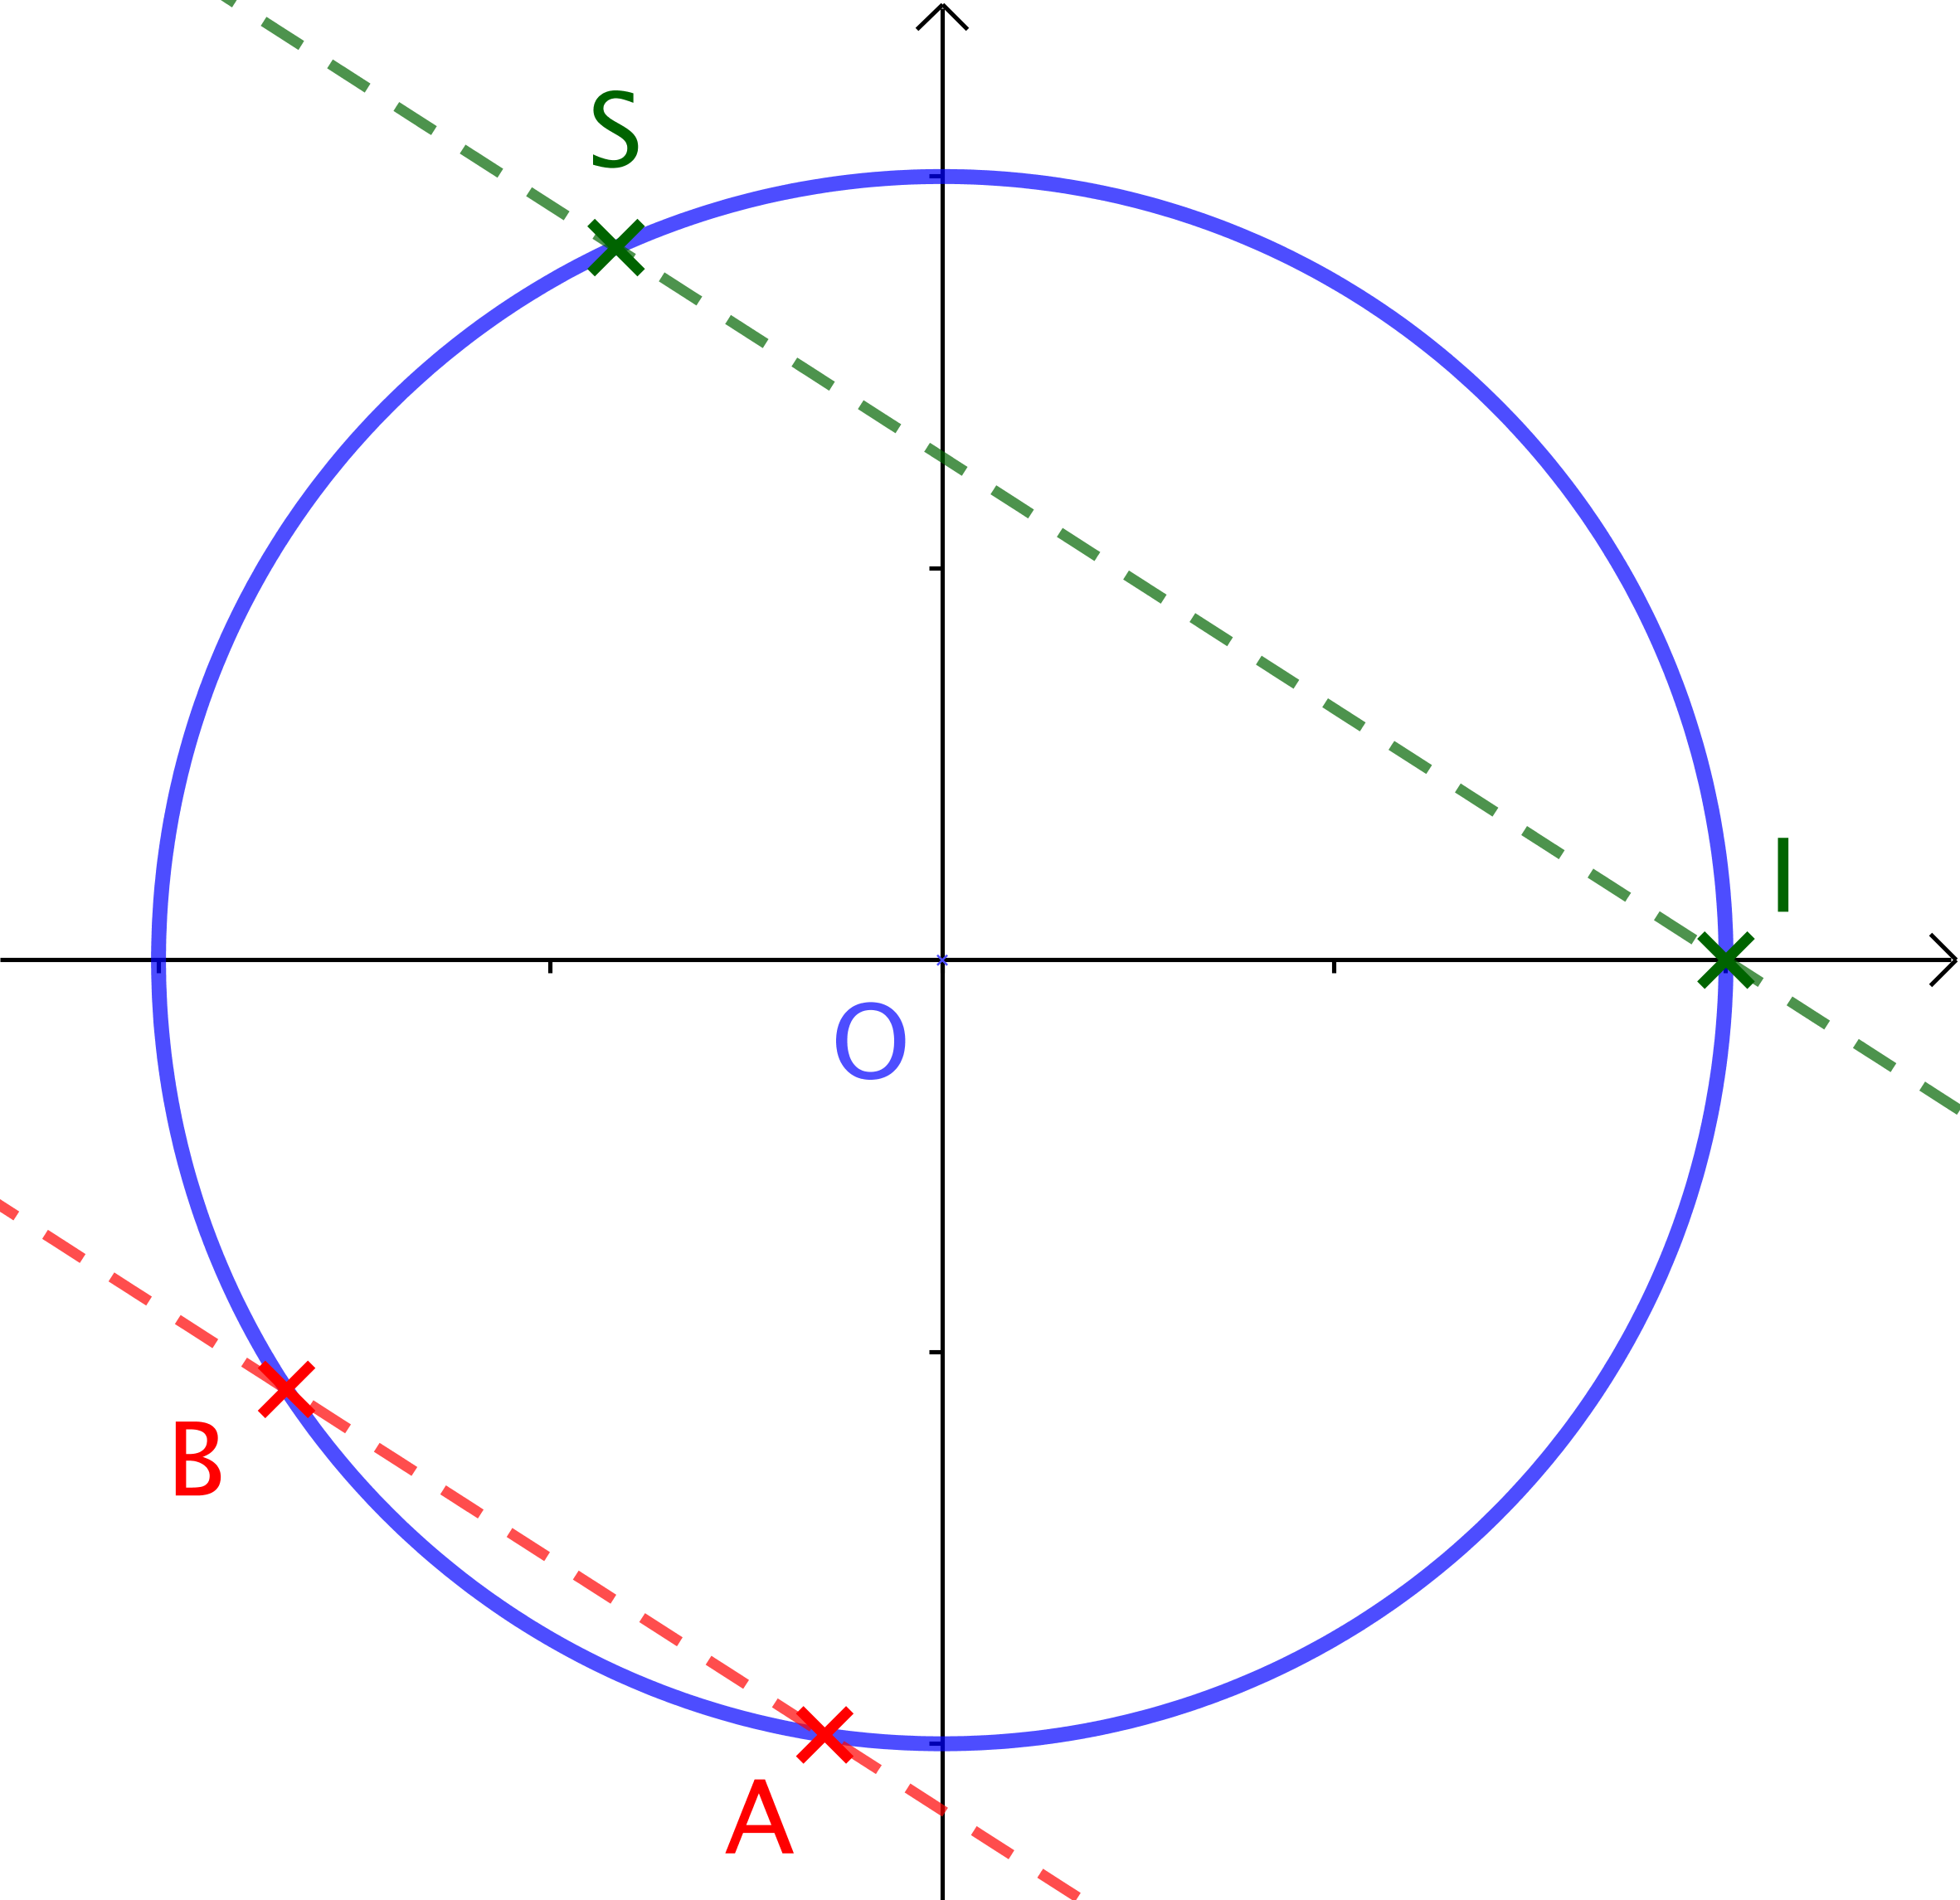
\includegraphics[scale = .6]{add-two-angles.png}}
\end{center}

\vspace{1em}


Nous avons alors que pour quatre points non nécessairement distincts $A$ , $B$ , $C$ et $D$ du cercle trigonométrique, si $\setgeo*{C}{AB} \,/\!/\,\setgeo*{C}{CD}$ alors
$\angleorient{\vect{OI}}{\vect{OA}} + \angleorient{\vect{OI}}{\vect{OB}} 
=
 \angleorient{\vect{OI}}{\vect{OC}} + \angleorient{\vect{OI}}{\vect{OD}}$ 
puisque les parallèles à $\setgeo*{C}{AB}$ et $\setgeo*{C}{CD}$ passant par $I$ sont confondues.
Avec ceci en tête, on peut alors analyser facilement la construction présentée au début du document.
Nous la redonnons ci-dessous pour le confort du lecteur où par hypothèse $n \in \NN_{\geq 5}$ .

\begin{enumerate}
	\item $\setgeo{D}\,'$ désigne la parallèle à $\setgeo*{C}{A_{n-3} A_{n-4}}$ passant par $A_{n-1}$ .

	\item Si $\setgeo{D}\,'$ est tangente au cercle alors $A_n \eq[def] A_{n-1}$ , sinon $A_n$ est le second point d'intersection de $\setgeo{D}\,'$ avec le cercle.
\end{enumerate}


\medskip

La construction est donc telle que $\forall n \in \NN_{\geq 5}$ , 
$\setgeo*{C}{A_{n} A_{n-1}} \,/\!/\, \setgeo*{C}{A_{n-3} A_{n-4}}$ 
\footnote{
	On peut définir $A_{n}$ comme étant l'unique point du cercle tel que $\setgeo*{C}{A_{n} A_{n-1}} \,/\!/\, \setgeo*{C}{A_{n-3} A_{n-4}}$  .
}.
Notant $\theta_i = \angleorient{\vect{OI}}{\vect{OA_i}}$ pour $i \in \NNs$ , nous avons alors
$\theta_i + \theta_{i+1} = \theta_{i+3} + \theta_{i+4}$ . Ceci nous donne les égalités suivantes :
\begin{itemize}[label=\small\textbullet]
	\item \textbf{[L1']} : 
	      $\theta_1 + \theta_{2} = \theta_{4} + \theta_{5}$

	\item \textbf{[L2']} : 
	      $\theta_2 + \theta_{3} = \theta_{5} + \theta_{6}$

	\item \textbf{[L3']} : 
	      $\theta_3 + \theta_{4} = \theta_{6} + \theta_{7}$
\end{itemize}


\medskip

Comme dans la première preuve, le système nous donne $\theta_1 = \theta_7$ . Sans plus d'effort, nous en déduisons que $A_7 = A_1$ . La beauté de cette preuve repose dans son côté presque automatique. La section \ref{group} révèlera toute la profondeur du raisonnement qui vient d'être fait, ce qui sera vraiment grandiose
\footnote{
	Ne jamais croire quelqu'un qui emploie trop de superlatifs.
} !
